\documentclass{article}
\usepackage{amsfonts}
\usepackage[utf8]{inputenc}
\usepackage{enumerate}
\usepackage{listings}
\usepackage{amsmath}
\usepackage{mathtools}
\usepackage{graphicx}
\usepackage[europeanresistors]{circuitikz}

\title{
    Progetto Demetra\\
    \large per sistemi di elettronica digitale \\
}
\author{Alessandro Lemme \\mat. 723923}
\date{\today}
\begin{document}
    \maketitle
    \section{Obiettivi del progetto}
    Programmare un circuito che tramite ESP32 DevKit e sensori sia in grado di:
    \begin{itemize}
        \item (ESP32) connettersi al wifi
        \item (DS1307) mantenere l'ora anche se disconnesso dalla rete o rimasto senza corrente
        \item che possa rilevare ed inviare dati ad un'api di un server in lan raccolti tramite:
        \begin{itemize}
            \item (FC-28) umidità del suolo
            \item (termistore) temperatura ambientale
            \item (fotoresistenza) intensità della luce
        \end{itemize}
        \item eventualmente connettersi ad un server esterno alla lan e recuperare l'ora usando i timestamp UNIX, per poi impostarla sul modulo RTC
    \end{itemize}
    \section{Struttura del codice}
    \begin{figure}
        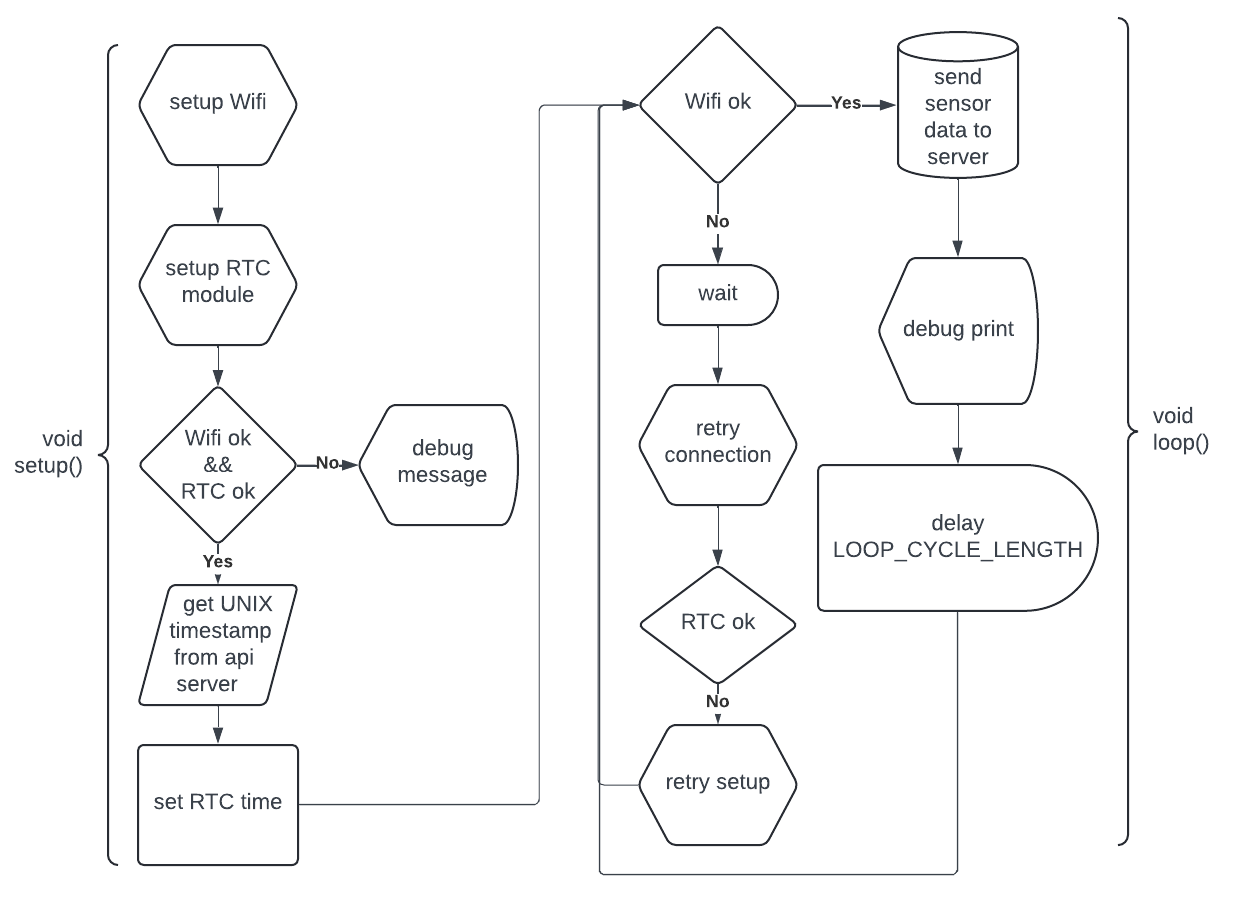
\includegraphics[width=\linewidth]{images/flow_chart.png}
        \caption{Flow chart di demetra.ino}
        \label{flow_chart}
    \end{figure}
    Il codice che viene eseguito dal microcontrollore è diviso in due sezioni; una che viene eseguita all'accensione della scheda (definito dalla funzione \texttt{void setup()}) ed una periodica (\texttt{void loop()}). \\
    All'accensione della scheda si ha la creazione dei servizi di base
    \subsection{Setup}

    \paragraph{Connessione al wifi} \texttt{setupWifi()}
    Usando la libreria \texttt{WiFi.h} si imposta la modalità del wifi come client (\texttt{WiFi.mode(WIFI\_STA)}) che si connette ad un router (al contrario di \texttt{WIFI\_AP} che lo rende un access point o di \texttt{WIFI\_AP\_STA} che lo rende un ripetitore). Si tenta quindi per un numero di volte pari alla costante \texttt{ALLOWED\_CONNECTION\_ATTEMPTS} (1 in questo caso) a connettersi al wifi. Lo stato del wifi (ottenibile con il getter \texttt{WiFi.status()}) può essere
    \begin{itemize}
        \item \texttt{WL\_CONNECTED} se si è connesso alla SSID correttamente 
        \item \texttt{WL\_NO\_SHIELD} se lo shield non è connesso correttamente alla scheda (difficile in questo caso) 
        \item \texttt{WL\_IDLE\_STATUS} temporaneo, mentre si sta connettendo 
        \item \texttt{WL\_CONNECT\_FAILED} se fallisce la connessione
        \item \texttt{WL\_NO\_SSID\_AVAIL} se non ci sono SSID rilevabili  
        \item \texttt{WL\_SCAN\_COMPLETED} al termine dello scan per delle reti  
        \item \texttt{WL\_CONNECTION\_LOST} se cade la connessione precedentemente stabilita con successo  
        \item \texttt{WL\_DISCONNECTED} alla disconnessione da una rete 
    \end{itemize}
    Nel caso la connessione abbia successo si stamperà sul monitor seriale una lista di dati; l'ip locale, la SSID a cui ci si è connessi e la qualità della connessione. Quest'ultima, la received signal strength information, il cui valore può essere letto tramite il metodo \texttt{WiFi.RSSI()} è un'unità di misura in decibell-milliwatts ($dBm$ o $dB_{mW}$), espressa usando una scala decibell rispetto ad un milliwatt; in formule, sia la potenza $P$ se misurata in $mW$ ed $x$ se misurata in $dBm$, allora
    \begin{align*}
        x & = 10 \log{\frac{P}{10^{-3}W}} \\
        P & = 10^{-3} \cdot 10^{\frac{x}{10}} \\
    \end{align*}


    \paragraph{Inizializzazione del modulo RTC} \texttt{RTC\_DS1307::begin$()$} Il modulo DS1307 è un orologio/calendario digitale a rappresentazione FBCD che usa un oscillatore a cristallo da $32.768kHz$ ed il protocollo $I^{2}C$ per la comunicazione. \\
    FBCD (fully coded binary decimal) significa che invece di usare un unico intero per rappresentare un dato momento - come nei timestamp UNIX, dove l'intero a 32bit indica i secondi trascorsi dall'1 gennaio 1970 - usa 4bit per rappresentare una singola cifra decimale. Questo modulo in particolare monta una nvSRAM da 54bit, utili quindi per rappresentare 14 cifre; 1 per l'indirizzo da cui iniziare a leggere/scrivere (\texttt{0x00} secondi, \texttt{0x02} minuti, ...), 2 ciascuno per secondi, minuti ed ore, 1 per il giorno della settimana e poi di nuovo 2 ciascuno per giorno, mese ed anno. \\
    Il protocollo $I^{2}C$ (inter integrated ciruit) è un sistema di comunicazione seriale bifilare usato tra circuiti integrati. In questo caso ci sono un solo master ed un solo slave, e si può comunicare con l'orologio usando la libreria \texttt{Wire.h}. Personalmente ho preferito usare la \texttt{RTCLib.h}, ma nel caso impostare la data sarebbe semplice, qui sotto un esempio di codice
    \begin{verbatim}
#include <Wire.h>

#define DS1307_ADDRESS 0x68

byte decToBcd(byte val) {
    return ( (val / 10 * 16) + (val % 10) );
}

void setDS1307Time(
    byte secondi, 
    byte minuti, 
    byte ore, 
    byte giorno, 
    byte data, 
    byte mese, 
    byte anno
) {
    Wire.beginTransmission(DS1307_ADDRESS);
    Wire.write(0);                  // Punto di partenza dell'array di registri
    Wire.write(decToBcd(secondi));  // Secondi (in BCD)
    Wire.write(decToBcd(minuti));   // Minuti (in BCD)
    Wire.write(decToBcd(ore));      // Ore (in BCD, formato 24 ore)
    Wire.write(decToBcd(giorno));   // Giorno della settimana (1=lunedì, 7=domenica)
    Wire.write(decToBcd(data));     // Giorno del mese (data)
    Wire.write(decToBcd(mese));     // Mese
    Wire.write(decToBcd(anno));     // Anno (0 = 2000, 21 = 2021)
    Wire.endTransmission();
}
    \end{verbatim}
    L'oscillatore a cristallo è un componente composto da un cristallo di quarzo (biossido di silicio - $SiO_{2}$), materiale piezoelettrico che in seguito a deformazione meccanica genera una tensione periodica (onda quadra) in questo caso convenientemente da $32.768kHz$ poichè divide un secondo in esattamente $2^{15}$ parti. La deformazione del cristallo avviene immergendolo in un campo elettrico ottenuto applicando una tensione ad un elettrodo per un dato periodo, al che il cristallo nel tornare alla sua forma iniziale inizierà a vibrare emettendo il segnale.  

    \paragraph{Connessione all'api del server per ottenere la data} \texttt{getServerTime$()$} e \texttt{RTC\_DS1307::adjust$($DateTime\ \&dt$)$} Se l'orologio viene inizializzato correttamente, e la connessione alla rete ha successo, allora utilizzando la libreria \texttt{HTTPClient.h} l'ESP32 creerà un oggetto \texttt{HTTPClient} e tramite il metodo \texttt{HTTPClient::begin} farà una richiesta \texttt{GET} ad un server esterno definito nella variabile \texttt{timeApiUri}, se avrà successo si avrà una stringa contenente il timestamp UNIX, che una volta convertito in \texttt{int}, e successivamente in \texttt{DateTime} potrà essere impostata sul modulo RTC utilizzando il metodo $I^{2}C$ di prima (anche se in \texttt{RTC\_DS1307.cpp} si usa \texttt{Adafruit\_I2CDevice} definita nella libreria omonima al posto di \texttt{Wire.h} come nel mio esempio di prima).

    \paragraph{Connessione all'api per il salvataggio dei dati registrati} \texttt{setupServerComunication$()$} Come ultima cosa del \texttt{setup()} se connesso alla lan il controllore tenterà di connettersi all'api HTTP di un server locale stabilendo una connessione TCP.

    \subsection{Loop} Terminato il setup si avrà il controllo periodico del funzionamento dell'orologio e dell'api, e nel caso di errore si tenterà di riconnettersi. Si avrà poi la raccolta dei dati da parte dei sensori quali;

    \paragraph{Temperatura con termistore} Il termistore è un resistore la cui resistenza varia al variare della temperatura. In questo progetto è stato fatto un partitore di tensione con un resistore da $100K\Omega$ e calcolata la sua resistenza $R_t$ con la forumula
    \begin{align*}
        R_{t} & = \frac{v_{out} \cdot R}{v_{in} - v_{out}}
    \end{align*}

    \begin{figure}[t] 
        \centering
        \begin{circuitikz}
            \ctikzset{resistor = american}
            \draw 
            (1.0, 0.0) 
            to[short, -o] (0.0, 0.0)
            to (1.0, 0.0) 
            to[R, label=$100K\Omega$] (3.0, 0.0)
            to[short, -o] (4.0, 0.0);
            \draw (3.0, 0.0) 
            to[thR] (3.0, -2.0)
            to (3.0, -2.0) node[ground]{};

            \node at (0.0, 0.0) [circ, draw=black, fill=white, thick, label=left:$V_{in}$] {};
            \node at (4.0, 0.0) [circ, draw=black, fill=white, thick, label=right:$V_{out}$] {};
            \node at (3.0, -2.0) [circ, draw=black, fill=white, thick, label=right:$Gnd$] {};
            \node at (1.0, 0.0) [circ] {};
            \node at (3.0, 0.0) [circ] {};
            \node at (3.0, -2.0) [circ] {};
        \end{circuitikz}
        \label{Partitore di tensione con termistore}
    \end{figure}
    La tensione viene misurata nel codice chiamando la funzione \texttt{analogRead(uint8\_t pin)} che ritornerà la tensione incognita $v_{out}$ su quel pin.

    \paragraph{Intensità della luce con fotoresistore} Analogamente al termistore la resistenza del fotoresistore è inversamente proporzionale alla quantità di luce che lo colpisce, tanto che la funzione che ricava la resistenza dei componenti è la stessa - \texttt{get\_voltage\_divider\_unknown\_resistance(...)}.

    \begin{figure}[h] 
        \centering
        \begin{circuitikz}
            \ctikzset{resistor = american}
            \draw 
            (1.0, 0.0) 
            to[short, -o] (0.0, 0.0)
            to (1.0, 0.0) 
            to[R, label=$100K\Omega$] (3.0, 0.0)
            to[short, -o] (4.0, 0.0);
            \draw (3.0, 0.0) 
            to[ldR] (3.0, -2.0)
            to (3.0, -2.0) node[ground]{};
            \node at (0.0, 0.0) [circ, draw=black, fill=white, thick, label=left:$V_{in}$] {};
            \node at (4.0, 0.0) [circ, draw=black, fill=white, thick, label=right:$V_{out}$] {};
            \node at (3.0, -2.0) [circ, draw=black, fill=white, thick, label=right:$Gnd$] {};
            \node at (1.0, 0.0) [circ] {};
            \node at (3.0, 0.0) [circ] {};
            \node at (3.0, -2.0) [circ] {};
        \end{circuitikz}
        \label{fig:Partitore di tensione con fotoresistore}
    \end{figure}

    \paragraph{Umidità del suolo} Il sensore FC-28 è misuratore di umidità del terreno resistivo; tanto più il terreno è secco tanto maggiore sarà la sua resistenza. E' composto da due componenti;
    \begin{itemize}
        \item Forche, da inserire nel terreno. Volendo si potrebbe usare anche un paio di cavi spelati \\
        \item PCB con potenziometro ed LM393, quest'ultimo compara due tensioni in ingresso e rende un'uscita digitale basata su quale tensione è maggiore. 
    \end{itemize}
    Di fatto segue lo stesso principio dei primi due sensori, ma ha l'extra dell' LM393.
    Al contrario un sensore basato su capacità è composto sempre da due elettrodi ma invece che misurare la tensione ai capi, con un NE555 o un TL555C si emette un'onda quadra; i due elettrodi saranno separati dal suolo che agirà da dielettrico, e tanto più sarà secco quanto più la sua capacità sarà minore. 
    \paragraph{Invio dei dati al server e controlli periodici} Tramite la connessione TCP di prima, si inviano i vari dati al server (nominato Ade). Dopo di che si attenderanno \texttt{LOOP\_CYCLE\_LENGTH} millisecondi. Ogni esecuzione del loop comporta anche un controllo sulla connessione alla rete, al server e al funzionamento dell'orologio. Ogni \texttt{CYCLES\_INTER\_WIF\_CONNECTION\_ATTEMPT} cicli senza connessione si ritenterà la connessione. Uguale per la connessione all'api ed all'orologio.

    \section{Extra: perché questi nomi?}
    Demetra era la dea greca della natura e dei raccolti. Questo è il nome del controllore che tiene controllate le piante.
    Ade era il dio greco dei morti, ma a me piace di più pensarlo come quello della memoria, dell'esperienza passata che non è più presente in un dato luogo; quando qualcosa non è più viene salvato da qualche altra parte perché non vada perso.
    Persefone era la figlia di Demetra e moglie di Ade, secondo il mito trascorreva i mesi autunnali ed invernali con suo marito, per poi essere restituita alla madre durante quelli primaverili ed estivi, per poi ripetere il ciclo. Questa figura mi sembrava un'analogia perfetta per gli scambi tra il server ed il controllore.

\end{document}